% ============================================================
% ANEXOS
% ============================================================

\appendix


% ============================================================
% ANEXO A
% ============================================================

\chapter{Ficha técnica del motor paso a paso}
\label{anexo:datasheet_motor}

En este anexo se presenta la ficha técnica del motor paso a paso
bifásico 17HS3401S utilizado como referencia para la parametrización
del modelo desarrollado en este trabajo.

Los principales parámetros empleados en el modelo se presentan en el
Capítulo~\ref{cap:Metodología}. La ficha técnica completa se incluye
a continuación con el propósito de respaldar los valores nominales
utilizados.

\begin{figure}[htbp]
    \centering
    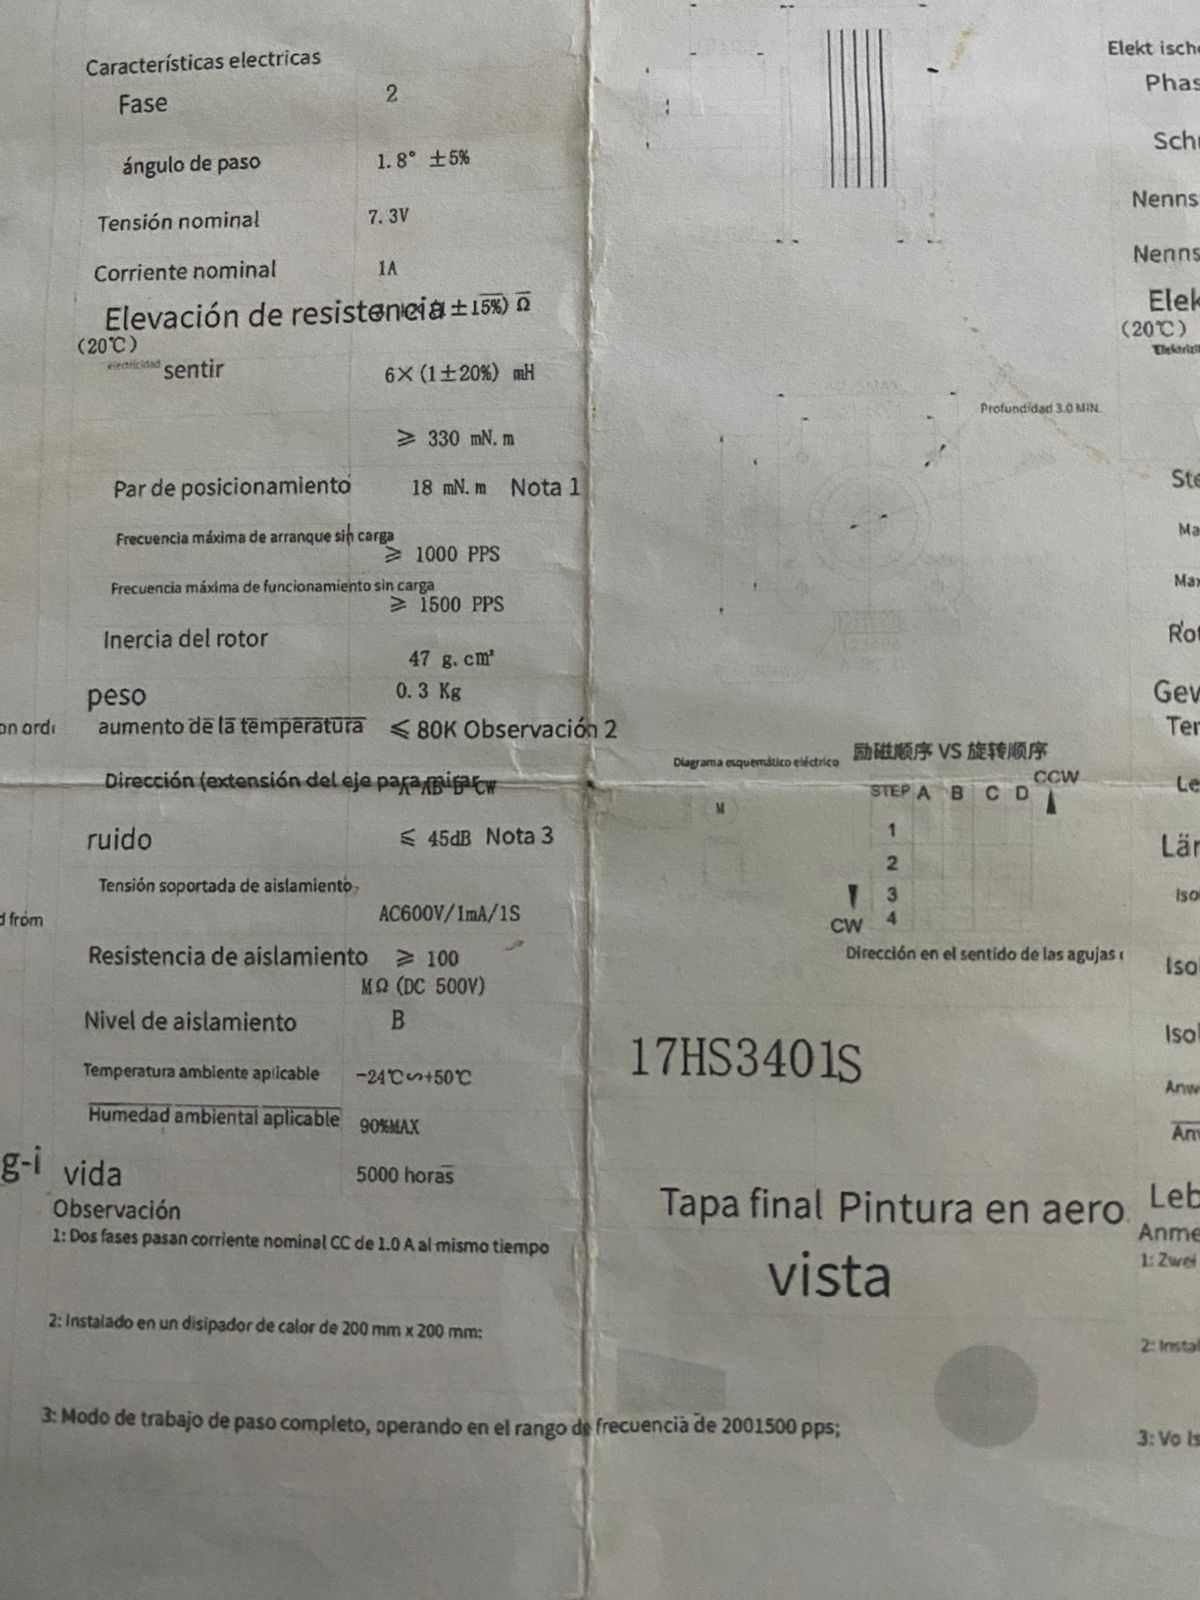
\includegraphics[
        width=0.85\textwidth,
        keepaspectratio
    ]{imagenes/anexos/datasheet_motor.png}
    \caption{Ficha técnica del motor paso a paso bifásico 17HS3401S.}
    \label{fig:datasheet_motor}
\end{figure}

\clearpage


% ============================================================
% ANEXO B
% ============================================================

\chapter{Caracterización experimental de la inductancia}
\label{anexo:medicion_inductancia}

Debido a la variación de la inductancia de fase con la posición del
rotor, se realizaron mediciones experimentales de inductancia sobre
el motor paso a paso bifásico 17HS3401S.

Estas mediciones fueron utilizadas para caracterizar la saliencia
magnética del motor y determinar los valores empleados posteriormente
para las inductancias asociadas a los ejes $d$ y $q$ del modelo.

La Figura~\ref{fig:medicion_inductancia} presenta el registro de las
mediciones realizadas.

\begin{figure}[htbp]
    \centering
    \includegraphics[
        width=0.85\textwidth,
        keepaspectratio
    ]{imagenes/anexos/medicion_inductancia.png}
    \caption{Registro de las mediciones de inductancia realizadas al
    motor paso a paso bifásico 17HS3401S.}
    \label{fig:medicion_inductancia}
\end{figure}


\section{Procedimiento de medición}
\label{anexo:procedimiento_inductancia}

La inductancia de las fases del motor fue medida para diferentes
posiciones del rotor con el propósito de identificar su variación
respecto de la posición mecánica.

% Completar posteriormente:
%
% - Instrumento utilizado.
% - Frecuencia de medición.
% - Condiciones de conexión.
% - Número de posiciones evaluadas.
% - Procedimiento utilizado para inmovilizar el rotor.
% - Incertidumbre o resolución del instrumento, si corresponde.


\section{Resultados de la caracterización}
\label{anexo:resultados_inductancia}

A partir de la caracterización experimental de la variación de
inductancia con la posición del rotor, se adoptaron para el modelo
los valores

\begin{equation}
    L_d = 3.66~\mathrm{mH},
\end{equation}

\begin{equation}
    L_q = 9.61~\mathrm{mH}.
\end{equation}

A partir de estos valores se definieron además la componente media
y la amplitud de variación de la inductancia como

\begin{equation}
    L_0 = \frac{L_d+L_q}{2}
        = 6.635~\mathrm{mH},
\end{equation}

\begin{equation}
    L_2 = \frac{L_q-L_d}{2}
        = 2.975~\mathrm{mH}.
\end{equation}

La diferencia entre ambas inductancias evidencia la existencia de
saliencia magnética, característica que posteriormente es considerada
en el modelo eléctrico del motor y en el análisis de estrategias de
estimación de posición basadas en inyección de señales de alta
frecuencia.

\clearpage


% ============================================================
% ANEXO C
% ============================================================

\chapter{Desarrollo matemático de los modelos de estimación}
\label{anexo:modelos_estimacion}

En este anexo se presentan los desarrollos matemáticos complementarios
asociados a los modelos de estado empleados para la estimación de las
variables mecánicas y de las perturbaciones.

En el cuerpo principal del documento se presentan las ecuaciones
necesarias para describir cada estrategia de estimación. Las
expresiones de mayor extensión se incluyen en este anexo con el
propósito de mantener la continuidad de la exposición.
% ------------------------------------------------------------
\section{Determinante de la matriz de inductancias}
\label{anexo:determinante_inductancias}

Para obtener las ecuaciones diferenciales de las corrientes de fase
es necesario invertir la matriz de inductancias del sistema bifásico,

\begin{equation}
    \mathbf{L}(\theta_e)=
    \begin{bmatrix}
        L_a & L_{ab} \\
        L_{ab} & L_b
    \end{bmatrix}.
\end{equation}

El determinante de esta matriz se define como

\begin{equation}
    \Delta_L
    =
    \det\left(\mathbf{L}(\theta_e)\right)
    =
    L_aL_b-L_{ab}^{2}.
\end{equation}

Considerando la dependencia de las inductancias con la posición
eléctrica del rotor,

\begin{align}
    L_a &= L_0 + L_2\cos(2\theta_e), \\
    L_b &= L_0 - L_2\cos(2\theta_e), \\
    L_{ab} &= L_2\sin(2\theta_e),
\end{align}

se obtiene

\begin{align}
    \Delta_L
    &=
    \left[L_0+L_2\cos(2\theta_e)\right]
    \left[L_0-L_2\cos(2\theta_e)\right]
    -
    L_2^2\sin^2(2\theta_e)
    \\
    &=
    L_0^2
    -
    L_2^2\cos^2(2\theta_e)
    -
    L_2^2\sin^2(2\theta_e)
    \\
    &=
    L_0^2
    -
    L_2^2
    \left[
        \cos^2(2\theta_e)
        +
        \sin^2(2\theta_e)
    \right]
    \\
    &=
    L_0^2-L_2^2.
\end{align}

Por otra parte, las componentes media y variable de la inductancia
se encuentran relacionadas con las inductancias en los ejes $d$ y
$q$ mediante

\begin{equation}
    L_0=\frac{L_d+L_q}{2},
    \qquad
    L_2=\frac{L_q-L_d}{2}.
\end{equation}

Por lo tanto,

\begin{align}
    \Delta_L
    &=
    \left(\frac{L_d+L_q}{2}\right)^2
    -
    \left(\frac{L_q-L_d}{2}\right)^2
    \\
    &=
    \frac{
        (L_d+L_q)^2-(L_q-L_d)^2
    }{4}
    \\
    &=
    \frac{4L_dL_q}{4}
    \\
    &=
    L_dL_q.
\end{align}

En consecuencia, para el modelo considerado,

\begin{equation}
    \boxed{
        \Delta_L=L_dL_q
    }.
\end{equation}

Utilizando los valores experimentales adoptados en este trabajo,

\begin{equation}
    L_d=3.66~\mathrm{mH},
    \qquad
    L_q=9.61~\mathrm{mH},
\end{equation}

se obtiene

\begin{equation}
    \Delta_L
    =
    (3.66\times10^{-3})
    (9.61\times10^{-3})
    \approx
    3.52\times10^{-5}~\mathrm{H^2}.
\end{equation}

Por consiguiente, $\Delta_L\neq0$ para los parámetros considerados,
por lo que la matriz de inductancias es invertible.

% ------------------------------------------------------------
\section{Modelo base de cuatro estados}
\label{anexo:modelo_4_estados}

El modelo base considera el vector de estados

\begin{equation}
    \mathbf{x}_4 =
    \begin{bmatrix}
        i_d &
        i_q &
        \omega_m &
        \theta_e
    \end{bmatrix}^{T}.
\end{equation}

De manera general, el sistema puede representarse como

\begin{equation}
    \dot{\mathbf{x}}_4 =
    \mathbf{f}_4(\mathbf{x}_4,\mathbf{u}),
\end{equation}

con una ecuación de medición

\begin{equation}
    \mathbf{y} =
    \mathbf{h}(\mathbf{x}_4,\mathbf{u}).
\end{equation}

% Insertar aquí, una vez cerrado el modelo:
%
% - ecuaciones completas de estado;
% - ecuaciones de salida;
% - entradas consideradas;
% - Jacobiano F;
% - Jacobiano H.


% ------------------------------------------------------------
\section{Modelo aumentado de cinco estados}
\label{anexo:modelo_5_estados}

Para incorporar el efecto de una perturbación mecánica desconocida,
el modelo base se amplía mediante un estado adicional $T_x$:

\begin{equation}
    \mathbf{x}_5 =
    \begin{bmatrix}
        i_d &
        i_q &
        \omega_m &
        \theta_e &
        T_x
    \end{bmatrix}^{T}.
\end{equation}

La dinámica del sistema aumentado puede expresarse como

\begin{equation}
    \dot{\mathbf{x}}_5 =
    \mathbf{f}_5(\mathbf{x}_5,\mathbf{u}).
\end{equation}

El estado $T_x$ representa una perturbación mecánica equivalente no
modelada explícitamente en el modelo nominal del accionamiento.

% Completar posteriormente:
%
% - dinámica adoptada para Tx;
% - ecuaciones completas;
% - Jacobiano del modelo aumentado;
% - ecuación de medición;
% - hipótesis utilizadas.


% ------------------------------------------------------------
\section{Modelo aumentado con componentes armónicas}
\label{anexo:modelo_armonico}

Con el propósito de representar componentes periódicas de la
perturbación, el modelo puede extenderse incorporando pares de estados
armónicos.

Para $H$ componentes armónicas, el vector de estados puede escribirse
de forma general como

\begin{equation}
    \mathbf{x}_{H} =
    \begin{bmatrix}
        i_d &
        i_q &
        \omega_m &
        \theta_e &
        T_x &
        A_1 &
        B_1 &
        \cdots &
        A_H &
        B_H
    \end{bmatrix}^{T}.
\end{equation}

Por lo tanto, la dimensión total del modelo es

\begin{equation}
    n_x = 5 + 2H.
\end{equation}

Cada componente armónica se representa mediante un par de estados
$A_h$ y $B_h$, cuya dinámica permite modelar una perturbación
periódica asociada a una frecuencia determinada.

Una representación general puede expresarse como

\begin{equation}
    \begin{bmatrix}
        \dot{A}_h \\
        \dot{B}_h
    \end{bmatrix}
    =
    \begin{bmatrix}
        0 & -\omega_h \\
        \omega_h & 0
    \end{bmatrix}
    \begin{bmatrix}
        A_h \\
        B_h
    \end{bmatrix},
\end{equation}

donde $\omega_h$ corresponde a la frecuencia angular asociada a la
componente armónica $h$.

% IMPORTANTE:
% Esta formulación deberá ajustarse a la implementación definitiva.
%
% Completar posteriormente:
%
% - relación entre omega_h y omega_m;
% - orden espacial del armónico;
% - ecuación de torque reconstruido;
% - Jacobiano completo;
% - tratamiento cuando omega_h depende de omega_m.

\clearpage


% ============================================================
% ANEXO D
% ============================================================

\chapter{Desarrollo del análisis de observabilidad}
\label{anexo:observabilidad}

En este anexo se presentan los desarrollos matemáticos complementarios
utilizados para evaluar la observabilidad de los diferentes modelos
de estado considerados en el trabajo.

La metodología general de análisis de observabilidad se presenta en
el marco teórico, mientras que los principales resultados y su
interpretación se desarrollan en el cuerpo principal del documento.


% ------------------------------------------------------------
\section{Observabilidad del modelo de cuatro estados}
\label{anexo:observabilidad_4}

Para el modelo

\begin{equation}
    \dot{\mathbf{x}} =
    \mathbf{f}(\mathbf{x},\mathbf{u}),
\end{equation}

\begin{equation}
    \mathbf{y} =
    \mathbf{h}(\mathbf{x}),
\end{equation}

la observabilidad local puede analizarse a partir de las derivadas de
Lie de las funciones de salida.

La derivada de Lie de primer orden se define como

\begin{equation}
    L_{\mathbf{f}}h =
    \frac{\partial h}{\partial \mathbf{x}}
    \mathbf{f}(\mathbf{x},\mathbf{u}).
\end{equation}

Las derivadas sucesivas se obtienen mediante

\begin{equation}
    L_{\mathbf{f}}^{k}h =
    \frac{\partial L_{\mathbf{f}}^{k-1}h}
    {\partial \mathbf{x}}
    \mathbf{f}(\mathbf{x},\mathbf{u}).
\end{equation}

A partir de estas expresiones se construye una matriz de observabilidad
local de la forma

\begin{equation}
    \mathcal{O}(\mathbf{x}) =
    \begin{bmatrix}
        \mathrm{d}h \\
        \mathrm{d}L_{\mathbf{f}}h \\
        \mathrm{d}L_{\mathbf{f}}^{2}h \\
        \vdots
    \end{bmatrix}.
\end{equation}

La condición de rango se evalúa respecto de la dimensión $n_x$ del
vector de estados.

% Insertar aquí:
%
% - matriz obtenida para el modelo de cuatro estados;
% - simplificaciones utilizadas;
% - condiciones particulares;
% - desarrollo simbólico completo si es necesario.


% ------------------------------------------------------------
\section{Observabilidad del modelo aumentado de cinco estados}
\label{anexo:observabilidad_5}

La incorporación del estado $T_x$ incrementa la dimensión del sistema
desde cuatro a cinco estados. En consecuencia, el análisis de
observabilidad debe considerar la capacidad de reconstruir tanto las
variables eléctricas y mecánicas como la perturbación equivalente.

% Insertar:
%
% O_5(x)
%
% Condiciones de rango.
%
% Casos:
%   - omega_m = 0
%   - omega_m != 0
%   - con saliencia
%   - sin saliencia
%
% No poner conclusiones largas aquí.
% Las conclusiones principales deben ir en Resultados.


% ------------------------------------------------------------
\section{Observabilidad del modelo con estados armónicos}
\label{anexo:observabilidad_armonica}

Para el modelo aumentado con $H$ componentes armónicas, la dimensión
del sistema corresponde a

\begin{equation}
    n_x = 5 + 2H.
\end{equation}

El análisis de observabilidad se realiza considerando la matriz
correspondiente al modelo aumentado y evaluando tanto su rango como
su condicionamiento numérico.

% Completar cuando estén disponibles los resultados definitivos.


% ------------------------------------------------------------
\section{Evaluación mediante valores singulares}
\label{anexo:valores_singulares}

Además de la condición de rango, se considera la descomposición en
valores singulares de la matriz de observabilidad,

\begin{equation}
    \mathcal{O}
    =
    U\Sigma V^{T},
\end{equation}

donde

\begin{equation}
    \Sigma =
    \operatorname{diag}
    \left(
        \sigma_1,
        \sigma_2,
        \ldots,
        \sigma_{n_x}
    \right).
\end{equation}

El menor valor singular,

\begin{equation}
    \sigma_{\min}(\mathcal{O}),
\end{equation}

permite complementar el análisis de rango al entregar información
sobre el condicionamiento de la reconstrucción de los estados.


% ------------------------------------------------------------
\section{Número de condición}
\label{anexo:condicion_observabilidad}

Cuando corresponda, el número de condición de la matriz de
observabilidad se calcula mediante

\begin{equation}
    \kappa(\mathcal{O})
    =
    \frac{\sigma_{\max}(\mathcal{O})}
         {\sigma_{\min}(\mathcal{O})}.
\end{equation}

Este indicador se utiliza como medida complementaria para identificar
situaciones en las cuales el sistema puede conservar rango completo,
pero presentar una observabilidad numéricamente débil.

\clearpage


% ============================================================
% ANEXO E
% ============================================================

\chapter{Jacobianos empleados en el estimador}
\label{anexo:jacobianos}

En este anexo se presentan los Jacobianos utilizados en la
implementación del estimador de estados.

Para un modelo no lineal de la forma

\begin{equation}
    \dot{\mathbf{x}}
    =
    \mathbf{f}(\mathbf{x},\mathbf{u}),
\end{equation}

el Jacobiano asociado a la dinámica se define como

\begin{equation}
    F =
    \frac{\partial \mathbf{f}}
         {\partial \mathbf{x}}.
\end{equation}

Por otra parte, para la ecuación de medición

\begin{equation}
    \mathbf{y}
    =
    \mathbf{h}(\mathbf{x},\mathbf{u}),
\end{equation}

el Jacobiano de medición corresponde a

\begin{equation}
    H =
    \frac{\partial \mathbf{h}}
         {\partial \mathbf{x}}.
\end{equation}


\section{Jacobiano del modelo de cuatro estados}
\label{anexo:jacobiano_4}

% Insertar F_4 y H_4 cuando estén cerrados.


\section{Jacobiano del modelo de cinco estados}
\label{anexo:jacobiano_5}

% Insertar F_5 y H_5 cuando estén cerrados.


\section{Jacobiano del modelo con estados armónicos}
\label{anexo:jacobiano_armonico}

% Insertar formulación general o las matrices correspondientes
% a la configuración finalmente utilizada.

\clearpage


% ============================================================
% ANEXO F
% ============================================================

\chapter{Parámetros de simulación y estimación}
\label{anexo:parametros_simulacion}

En este anexo se presentan los parámetros complementarios utilizados
en las simulaciones y en los algoritmos de estimación. Los parámetros
fundamentales para comprender y reproducir los experimentos se
presentan también en el cuerpo principal del documento.
\section{Frecuencias y tiempos de muestreo}

\begin{table}[htbp]
    \centering
    \caption{Frecuencias y tiempos de muestreo utilizados.}
    \label{tab:tiempos_muestreo}
    \begin{tabular}{lcc}
        \hline
        \textbf{Subsistema} &
        \textbf{Frecuencia} &
        \textbf{Tiempo de muestreo} \\
        \hline
        Portadora PWM          & 20 kHz & 50 $\mu$s \\
        Control de corriente   & 10 kHz & 100 $\mu$s \\
        EKF                    & 10 kHz & 100 $\mu$s \\
        Control de velocidad   & 1 kHz  & 1 ms \\
        Control de posición    & 100 Hz & 10 ms \\
        \hline
    \end{tabular}
\end{table}

\section{Parámetros del controlador de corriente}

\begin{table}[htbp]
    \centering
    \caption{Parámetros del controlador de corriente en ejes $dq$.}
    \label{tab:parametros_control_corriente}
    \begin{tabular}{lcc}
        \hline
        \textbf{Parámetro} & \textbf{Valor} & \textbf{Unidad} \\
        \hline
        Ancho de banda eje $d$ & 500 & Hz \\
        Ancho de banda eje $q$ & 500 & Hz \\
        Frecuencia de ejecución & 10000 & Hz \\
        Tensión del bus DC & 24 & V \\
        Corriente máxima & 2.404 & A \\
        \hline
    \end{tabular}
\end{table}

\section{Parámetros del modelo del motor}

% Completar/ajustar cuando cierres definitivamente los valores.

\begin{table}[htbp]
    \centering
    \caption{Parámetros utilizados en el modelo del motor paso a paso.}
    \label{tab:parametros_motor_anexo}
    \begin{tabular}{lccc}
        \hline
        \textbf{Parámetro} &
        \textbf{Símbolo} &
        \textbf{Valor} &
        \textbf{Unidad} \\
        \hline
        Ángulo de paso              & $\alpha_s$ & 1.8 & $^\circ$ \\
        Número de fases             & $N_{ph}$   & 2 & -- \\
        Pasos por revolución        & $N_s$      & 200 & -- \\
        Número de dientes           & $N_t$      & 100 & -- \\
        Pares de polos              & $P$        & 50 & -- \\
        Corriente nominal           & $I_{nom}$  & 1.7 & A \\
        Corriente máxima            & $I_{max}$  & 2.404 & A \\
        Torque de detención         & $T_{dm}$   & 0.022 & N\,m \\
        Torque de retención         & $T_{hold}$ & 0.392 & N\,m \\
        Constante de torque         & $K_t$      & 0.1631 & N\,m/A \\
        Flujo equivalente           & $\Psi$     & $3.261\times10^{-3}$ & Wb \\
        Resistencia de fase         & $R$        & 2.5 & $\Omega$ \\
        Inductancia nominal         & $L$        & 6.0 & mH \\
        Inductancia eje $d$         & $L_d$      & 3.66 & mH \\
        Inductancia eje $q$         & $L_q$      & 9.61 & mH \\
        Inductancia media           & $L_0$      & 6.635 & mH \\
        Amplitud de variación       & $L_2$      & 2.975 & mH \\
        Inercia interna             & $J$        & $5.4\times10^{-6}$ & kg\,m$^2$ \\
        Fricción viscosa interna    & $B$        & $1\times10^{-4}$ & N\,m\,s/rad \\
        Fricción de Coulomb         & $T_c$      & 0.002 & N\,m \\
        Fase del cogging            & $\phi$     & $\pi/2$ & rad \\
        \hline
    \end{tabular}
\end{table}

\section{Parámetros del EKF}
\label{anexo:parametros_ekf}

% Incorporar aquí las matrices definitivas:
%
% Q
% R
% P_0
% Ts
%
% Evitar poner valores preliminares hasta cerrar la sintonización.


\section{Parámetros de la inyección de alta frecuencia}
\label{anexo:parametros_hfi}

\begin{table}[htbp]
    \centering
    \caption{Parámetros empleados para la inyección de alta frecuencia.}
    \label{tab:parametros_hfi}
    \begin{tabular}{lccc}
        \hline
        \textbf{Parámetro} &
        \textbf{Símbolo} &
        \textbf{Valor} &
        \textbf{Unidad} \\
        \hline
        Amplitud de inyección & $V_h$ & 2 & V \\
        Frecuencia de inyección & $f_h$ & 2000 & Hz \\
        Ancho de banda BPF & $BW_{HFI}$ & 25 & Hz \\
        Frecuencia de procesamiento & $f_s$ & 10000 & Hz \\
        \hline
    \end{tabular}
\end{table}


\section{Parámetros del controlador resonante}
\label{anexo:parametros_pr}

% Completar:
%
% - Kp;
% - Kr;
% - ancho de banda;
% - frecuencia resonante;
% - límites de saturación;
% - estrategia de actualización de omega_r.